
\documentclass[sigplan,nonacm]{acmart}

\settopmatter{printacmref=false}
\setcopyright{none}
\renewcommand\footnotetextcopyrightpermission[1]{}

\usepackage{amsmath}
\usepackage{booktabs}
\usepackage{pgfplots}
\usepackage{tikz}
\usepackage{xurl}
\usepackage{listings}
\usepackage{placeins}

\pgfplotsset{compat=1.18}
\usetikzlibrary{arrows.meta,positioning}

\setlength{\textfloatsep}{8pt plus 2pt minus 2pt}
\setlength{\floatsep}{6pt plus 2pt minus 2pt}
\setlength{\intextsep}{6pt plus 2pt minus 2pt}
\setlength{\abovecaptionskip}{3pt}
\setlength{\belowcaptionskip}{2pt}
\emergencystretch=2em

\definecolor{fc}{RGB}{55,89,150}
\definecolor{qo}{RGB}{29,145,119}
\definecolor{aone}{RGB}{210,139,48}
\definecolor{afive}{RGB}{137,95,175}
\definecolor{hy}{RGB}{185,75,99}

\pgfplotsset{
comp/.style={
width=\columnwidth,
height=3.45cm,
ybar,
bar width=5pt,
symbolic x coords={Fairness,Balanced},
xtick=data,
enlarge x limits=.27,
grid=major,
grid style={gray!13},
tick label style={font=\scriptsize},
label style={font=\scriptsize},
legend style={
font=\tiny,
draw=none,
fill=none,
at={(.5,-.23)},
anchor=north,
legend columns=5,
/tikz/every even column/.append style={
column sep=2pt
}
}
}
}

\lstset{
basicstyle=\ttfamily\scriptsize,
breaklines=true,
columns=fullflexible,
frame=single,
showstringspaces=false
}

\title{
Length-Aware Request Scheduling for vLLM:
Performance and Fairness Trade-offs in LLM Serving
}

\author{Carleano Chang (poching2)}
\author{Christine Liou (ycliou2)}

\renewcommand{\shortauthors}{Chang and Liou}

\begin{document}

\begin{abstract}
LLM inference requests vary in prompt and generation
length, creating latency and fairness challenges under
constrained GPU capacity. We implement four lightweight
length-aware waiting-queue policies in vLLM and compare
them with native first-come, first-served (FCFS)
scheduling. Across two 900-request GPU workloads and
38 primary runs, Queue-Only scheduling reduces
short-request P95 time to first token (TTFT) by
94.2\% and 99.2\%, respectively. In the short-heavy
workload, however, long-request P95 TTFT increases
from 10.056 to 19.012 seconds. Our results show that
queue reordering can substantially improve short-request
responsiveness while introducing workload-dependent
fairness trade-offs.
\end{abstract}

\keywords{
LLM serving, vLLM, scheduling,
tail latency, fairness
}

\maketitle

\pagestyle{plain}
\thispagestyle{plain}

% ============================================================
% 1. INTRODUCTION
% ============================================================

\section{Introduction}

Interactive LLM services process requests with widely
varying input and output lengths. When GPU capacity is
limited, requests compete for admission, and a long
request can delay a much shorter one.

vLLM improves serving efficiency using PagedAttention
and continuous batching~\cite{kwon2023efficient},
but efficient execution does not remove the need
to choose which waiting requests to prioritize.

We ask:
\emph{Can lightweight length-aware queue ordering
improve short-request tail latency without unacceptable
losses in long-request latency or throughput?}

We implement four policies on top of vLLM's native
scheduler, evaluate them under short-heavy and
balanced traffic, and analyze latency, throughput,
and fairness.

Our contribution is a controlled comparison of
queue-priority heuristics rather than a replacement
for the GPU execution or batching engine.

An important distinction is that a scheduling policy
can improve responsiveness for one class of requests
without improving the experience of every request.
We therefore evaluate short and long requests
separately instead of relying only on aggregate
latency measurements.

% ============================================================
% 2. RELATED WORK
% ============================================================

\section{Related Work}

\textbf{vLLM.}
Kwon et al.~\cite{kwon2023efficient} introduced
PagedAttention to manage KV-cache memory efficiently,
improving concurrent LLM serving. We retain vLLM's
memory management and batching, changing only
waiting-request ordering.

\textbf{Orca.}
Yu et al.~\cite{yu2022orca} proposed iteration-level
scheduling and selective batching for variable-length
transformer generation. Our intervention is narrower:
it changes priorities before native scheduling rather
than redesigning batching.

\textbf{Sarathi-Serve.}
Agrawal et al.~\cite{agrawal2024sarathi} studied
throughput--latency trade-offs using techniques
including chunked prefill.

Our experiments examine a complementary trade-off:
the effect of prioritizing estimated-short requests
on short and long tail latency.

Unlike these systems, our policies cannot guarantee
execution order or starvation freedom.

The comparison motivates a deliberately lightweight
design: we preserve the serving engine and isolate
waiting-queue priority as the main experimental
variable.

% ============================================================
% 3. TECHNICAL APPROACH
% ============================================================

\section{Technical Approach}

\subsection{Priority Functions}

For request $i$, let $p_i$ be prompt tokens,
$o_i$ the requested maximum output tokens,
and $w_i(t)$ its elapsed waiting time.

We estimate request size as

\begin{equation}
L_i=p_i+o_i,\qquad
w_i(t)=\max(0,t-a_i),
\end{equation}

where $a_i$ is its arrival time.

This is an inexpensive proxy for work, not an exact
runtime prediction: prefill and decoding have
different costs, and actual output may be shorter
than the limit.

We compare five policies.

\textbf{Native FCFS}
retains vLLM's default queue ordering.

\textbf{Queue-Only}
sorts waiting requests by ascending $L_i$,
prioritizing short requests without considering
waiting time.

\textbf{Aging}
uses

\begin{equation}
P_i(t)=
\frac{L_i}{1+\alpha w_i(t)},
\quad
\alpha\in\{0.1,0.5\}.
\label{eq:aging}
\end{equation}

A lower score receives higher priority; older
requests gradually become more competitive.

\textbf{Hybrid}
delays the aging effect until $d=5$ seconds:

\begin{equation}
P_i(t)=
\frac{L_i}{
1+0.5\max(0,w_i(t)-5)
}.
\label{eq:hybrid}
\end{equation}

Before five seconds, Hybrid behaves like
Queue-Only; afterward, waiting time lowers
the score.

These are heuristics and do not provide
formal waiting-time bounds.

\subsection{Design Rationale}

Queue-Only serves as a simple length-aware baseline.
Its advantage is that it requires no additional
waiting-time parameter.

Aging introduces a mechanism for increasing the
relative priority of requests that remain queued.
The two values of $\alpha$ allow us to compare
different aging strengths.

Hybrid delays this adjustment to preserve the
initial short-request preference while giving
older requests an opportunity to gain priority.

These alternatives help determine whether
additional fairness-oriented heuristics provide
measurable benefits over simple length ordering.

\subsection{Priority Score Interpretation}

The aging formula creates a trade-off between
estimated request size and elapsed waiting time.
For two requests, an older long request can move
ahead of a newer short request when its discounted
priority score becomes smaller.

However, increasing $\alpha$ does not uniformly
favor long requests: both requests receive a
waiting-time adjustment, and their relative order
depends on their individual ages and lengths.

The Hybrid policy introduces another boundary.
Requests waiting less than five seconds receive
no aging adjustment, while older requests begin
receiving a progressively lower priority score.

This behavior motivates evaluating actual
tail-latency outcomes rather than assuming that
a more aggressive aging parameter always
improves fairness.

\subsection{Integration and Complexity}

Our custom scheduler reorders vLLM's
\texttt{waiting} and
\texttt{skipped\_waiting} queues before invoking
the parent \texttt{schedule()} method.

Native vLLM still controls batching,
memory constraints, and GPU admission.

Priority computation costs $O(n)$ for $n$
waiting requests; comparison sorting costs
$O(n\log n)$ per reordering.

End-to-end effects also depend on queue length,
scheduling frequency, and the underlying
inference engine.

Appendix~\ref{app:example} illustrates all
five policies with concrete requests.

% ============================================================
% 4. IMPLEMENTATION DETAILS
% ============================================================

\section{Implementation Details}

\subsection{Components and Prior Analysis}

The project separates four major components:

(1) JSONL workload generation,
(2) custom queue-ordering schedulers,
(3) an asynchronous streaming benchmark client,
and (4) offline statistical analysis.

Before GPU evaluation, we implemented preliminary
CPU tests and small smoke tests to validate
request generation, scheduling integration,
and measurement collection.

The formal GPU experiments use the same benchmark
concepts but a separate GPU environment.

The benchmark client submits requests according
to recorded arrival times and logs submission,
first-token, and completion timestamps,
token counts, and errors.

Per-request observations are saved as
\texttt{raw\_results.jsonl}; aggregate results
are saved as \texttt{summary.json}.

This makes it possible to inspect request-level
behavior and regenerate summary plots.

\subsection{Workloads, Metrics, and Tests}

Two Poisson-arrival workloads each contain
900 requests at a target rate of 30 requests/s.

Short requests use approximately 32 prompt
and 16 output tokens; long requests use
approximately 256 prompt and 128 output tokens.

The fairness mix has 813 short and 87 long
requests; the balanced mix has 455 short
and 445 long requests.

For request $i$,

\begin{equation}
\mathrm{TTFT}_i=
t_i^{\mathrm{first}}-t_i^{\mathrm{send}}.
\end{equation}

We report separate short- and long-request
P95 TTFT and generated output-token throughput,
defined as output tokens divided by benchmark
duration.

TTFT includes queueing and initial server
processing, so it is not a direct measure
of queue delay.

The repository contains 46 passing unit tests
covering workload generation, metrics,
result processing, and scheduler logic.

Smoke tests check end-to-end integration;
900-request workloads exercise the system
under sustained arrivals.

The generator, client, policies, and offline
analysis work for the evaluated configuration.

Formal starvation guarantees and exhaustive
compatibility with other vLLM versions
are not established.

\subsection{Measurement Reliability}

We retain both aggregate summaries and raw
request-level measurements rather than relying
only on a single reported average.

Repeated benchmark runs help expose variation
caused by arrival timing, queue interactions,
and shared GPU activity.

The analysis pipeline also records run-selection
decisions, allowing anomalous measurements
to be examined without silently removing them.

This is particularly important for tail latency,
where a relatively small number of delayed
requests can influence the P95 result.

\subsection{Experimental Control}

The two workloads use the same request-count
and target-arrival-rate settings, but differ
in the proportion of short and long requests.

This separates workload composition from
overall request count when interpreting the
results.

Each policy is evaluated using the same
definitions of TTFT and throughput, and
run-level measurements are summarized using
the same analysis procedure.

Nevertheless, execution on a shared GPU
introduces possible environmental variation.
Repeated runs reduce reliance on a single
measurement but do not eliminate this
source of uncertainty.

\subsection{Artifact Layout and Execution}

Source and documentation:

\url{https://github.com/Car1eano/fall26-cs598ape-llm-length-aware-scheduling}

Scheduler implementations and preserved GPU
results are in \texttt{gpu\_experiments/};
the client is in \texttt{benchmarks/};
tests are in \texttt{tests/};
plots and statistical scripts are in
\texttt{report\_analysis/}.

Run unit tests with

\begin{center}
\texttt{python -m pytest tests/ -v}
\end{center}

The benchmark client accepts a workload JSONL
file, model, server URL, and output directory.

Appendix~\ref{app:repro} gives exact commands
and reproduction limitations.

% ============================================================
% 5. EXPERIMENTAL RESULTS
% ============================================================

\section{Experimental Results}

\subsection{Setup and Main Measurements}

We evaluate
\texttt{Qwen/Qwen2.5-0.5B-Instruct}
with vLLM 0.26.0 on a shared
NVIDIA GeForce RTX 5090.

The dataset comprises 38 primary GPU runs
and two retained diagnostic runs.

Tables~\ref{tab:fair} and~\ref{tab:bal}
report means of run-level metrics;
P95 values are calculated per run
before averaging.

The number of runs varies by policy.

\begin{table}[t]
\centering
\caption{
Fairness workload (813 short, 87 long).
P95 TTFT in seconds.
}
\label{tab:fair}
\scriptsize
\setlength{\tabcolsep}{3pt}
\begin{tabular}{lrrrr}
\toprule
Policy & $n$ & Tok/s & Short P95 & Long P95\\
\midrule
FCFS & 3 & 573.74 & 10.107 & 10.056\\
Queue-Only & 5 & 561.64 & 0.590 & 19.012\\
Aging 0.1 & 3 & 553.64 & 0.644 & 19.551\\
Aging 0.5 & 5 & 573.04 & 0.680 & 18.266\\
Hybrid & 3 & 560.01 & 0.629 & 18.880\\
\bottomrule
\end{tabular}
\end{table}

\begin{table}[t]
\centering
\caption{
Balanced workload (455 short, 445 long).
P95 TTFT in seconds.
}
\label{tab:bal}
\scriptsize
\setlength{\tabcolsep}{3pt}
\begin{tabular}{lrrrr}
\toprule
Policy & $n$ & Tok/s & Short P95 & Long P95\\
\midrule
FCFS & 3 & 577.49 & 79.310 & 77.468\\
Queue-Only & 5 & 582.80 & 0.664 & 77.282\\
Aging 0.1 & 3 & 571.43 & 0.721 & 79.618\\
Aging 0.5 & 5 & 585.54 & 1.322 & 76.815\\
Hybrid & 3 & 556.50 & 6.315 & 82.219\\
\bottomrule
\end{tabular}
\end{table}

\subsection{Short-Request Responsiveness}

Figure~\ref{fig:short} shows that every
length-aware policy improves short-request
P95 TTFT relative to FCFS.

In the fairness workload, Queue-Only reduces
P95 TTFT from 10.107 to 0.590 seconds,
a 94.2\% reduction.

In balanced traffic, the reduction is from
79.310 to 0.664 seconds, or 99.2\%.

Queue-Only achieves the lowest short-request
P95 in both workloads.

This is consistent with earlier admission
consideration for short requests, although
TTFT does not isolate pure queueing delay.

\begin{figure}[t]
\centering
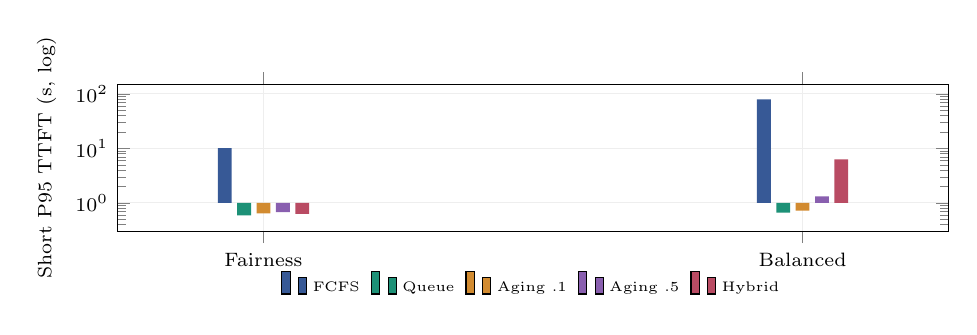
\begin{tikzpicture}
\begin{axis}[
comp,
ymode=log,
log basis y=10,
ymin=.3,
ymax=150,
ylabel={Short P95 TTFT (s, log)}
]
\addplot[fill=fc,draw=none]
coordinates {
(Fairness,10.107)
(Balanced,79.310)
};
\addplot[fill=qo,draw=none]
coordinates {
(Fairness,.590)
(Balanced,.664)
};
\addplot[fill=aone,draw=none]
coordinates {
(Fairness,.644)
(Balanced,.721)
};
\addplot[fill=afive,draw=none]
coordinates {
(Fairness,.680)
(Balanced,1.322)
};
\addplot[fill=hy,draw=none]
coordinates {
(Fairness,.629)
(Balanced,6.315)
};
\legend{
FCFS,Queue,Aging .1,Aging .5,Hybrid
}
\end{axis}
\end{tikzpicture}
\caption{
Short-request P95 TTFT.
Lower is better; logarithmic scale.
}
\Description{
Short-request P95 TTFT across
five scheduling policies.
}
\label{fig:short}
\end{figure}

\subsection{Long-Request Fairness}

The short-heavy workload exposes a clear cost.

Queue-Only increases long-request P95 TTFT
from 10.056 to 19.012 seconds,
approximately an 89\% increase.

Aging 0.1, Aging 0.5, and Hybrid also increase
long-request tail latency relative to FCFS.

In balanced traffic, long-request P95
remains near 77--82 seconds across policies.

Thus, the fairness cost of length-aware
scheduling depends on workload composition
and should not be inferred from short-request
improvements alone.

\begin{figure}[t]
\centering
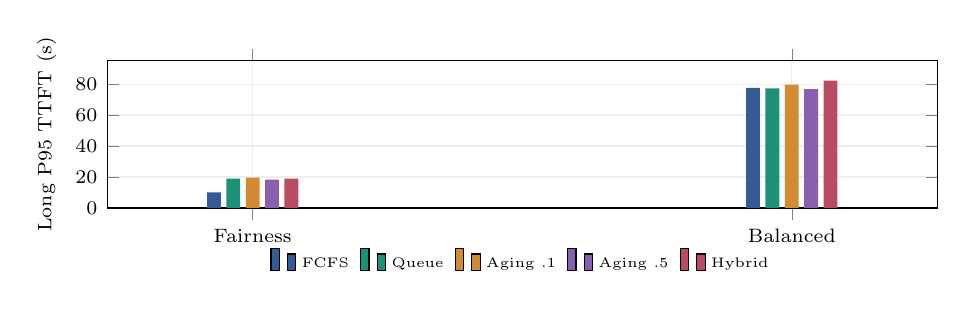
\begin{tikzpicture}
\begin{axis}[
comp,
ymin=0,
ymax=95,
ylabel={Long P95 TTFT (s)}
]
\addplot[fill=fc,draw=none]
coordinates {
(Fairness,10.056)
(Balanced,77.468)
};
\addplot[fill=qo,draw=none]
coordinates {
(Fairness,19.012)
(Balanced,77.282)
};
\addplot[fill=aone,draw=none]
coordinates {
(Fairness,19.551)
(Balanced,79.618)
};
\addplot[fill=afive,draw=none]
coordinates {
(Fairness,18.266)
(Balanced,76.815)
};
\addplot[fill=hy,draw=none]
coordinates {
(Fairness,18.880)
(Balanced,82.219)
};
\legend{
FCFS,Queue,Aging .1,Aging .5,Hybrid
}
\end{axis}
\end{tikzpicture}
\caption{
Long-request P95 TTFT.
Lower is better.
}
\Description{
Long-request P95 TTFT across
five scheduling policies.
}
\label{fig:long}
\end{figure}

\subsection{Aging and Throughput Trade-offs}

Aging does not consistently outperform
Queue-Only.

Under fairness traffic, Aging 0.5 has slightly
lower long-request P95 TTFT
(18.266 vs. 19.012 seconds),
but slightly higher short-request P95 TTFT
(0.680 vs. 0.590 seconds).

In balanced traffic, Hybrid's short P95
is 6.315 seconds, worse than the other
length-aware variants.

Stronger aging therefore does not guarantee
better measured fairness or responsiveness.

Figure~\ref{fig:throughput} shows that throughput
differences are smaller than latency changes.

Queue-Only is approximately 2.1\% below FCFS
in fairness traffic
(561.64 vs. 573.74 tokens/s)
and 0.9\% above it in balanced traffic
(582.80 vs. 577.49 tokens/s).

These small differences should not be treated
as statistically significant without
uncertainty estimates.

\begin{figure}[t]
\centering
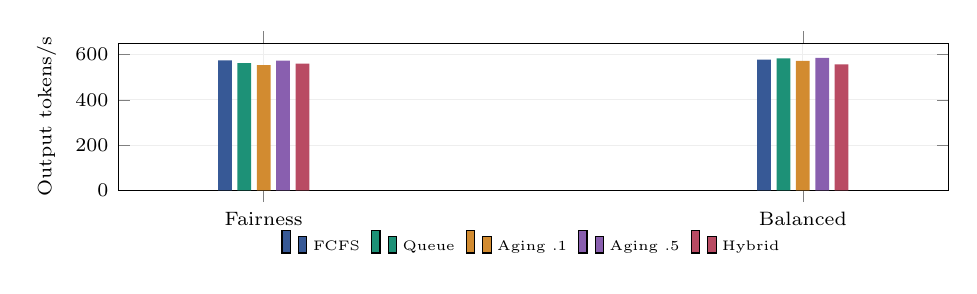
\begin{tikzpicture}
\begin{axis}[
comp,
ymin=0,
ymax=650,
ylabel={Output tokens/s}
]
\addplot[fill=fc,draw=none]
coordinates {
(Fairness,573.74)
(Balanced,577.49)
};
\addplot[fill=qo,draw=none]
coordinates {
(Fairness,561.64)
(Balanced,582.80)
};
\addplot[fill=aone,draw=none]
coordinates {
(Fairness,553.64)
(Balanced,571.43)
};
\addplot[fill=afive,draw=none]
coordinates {
(Fairness,573.04)
(Balanced,585.54)
};
\addplot[fill=hy,draw=none]
coordinates {
(Fairness,560.01)
(Balanced,556.50)
};
\legend{
FCFS,Queue,Aging .1,Aging .5,Hybrid
}
\end{axis}
\end{tikzpicture}
\caption{
Mean output-token throughput.
Higher is better.
}
\Description{
Output-token throughput across
five scheduling policies.
}
\label{fig:throughput}
\end{figure}

One original Queue-Only fairness run
had unusually low throughput.

We preserved the result and audited original,
retest, and combined selections rather than
silently discarding it.

The short-request latency conclusion remains
stable across selections, whereas throughput
is more sensitive; Appendix~\ref{app:sensitivity}
reports the values.

\subsection{Threats to Validity}

Our conclusions are limited by one relatively
small model, two synthetic workload mixes,
a small number of repeated runs,
and shared GPU infrastructure.

Estimated length is not actual service time,
and neither aging nor hybrid priority
proves starvation freedom.

Exact formal GPU launch settings have not
been packaged into a verified one-command
rerun; preserved request-level logs
support offline analysis.

\subsection{Interpretation of the Workload Difference}

The two traffic mixes lead to different
baseline queueing behavior.

With only 87 long requests in the fairness
workload, FCFS gives short and long classes
similar P95 TTFT
(10.107 and 10.056 seconds).

Length prioritization changes which class
receives early admission: short P95 falls
below one second, while long P95 rises
to approximately 18--20 seconds.

This is a latency redistribution,
not an across-the-board improvement.

Under balanced traffic, FCFS gives both
classes much higher P95 TTFT
(79.310 and 77.468 seconds).

Length-aware ordering sharply reduces
short P95 while long P95 stays near
its original level.

The results should not be interpreted
as proving that a balanced workload
is universally more favorable:
queue state, admission capacity,
and model configuration also
influence the outcome.

\subsection{What the Aging Results Establish}

Aging is intended to protect requests
that have waited for a long time,
but our measurements do not establish
a monotonic relationship between
aging strength and fairness.

In the fairness workload, Aging 0.1
has a long-request P95 of 19.551 seconds,
while Aging 0.5 gives 18.266 seconds;
Queue-Only gives 19.012 seconds.

These values show a small trade-off,
not a guarantee.

In balanced traffic, Aging 0.5 produces
the highest mean throughput
(585.54 tokens/s), yet Queue-Only still
has the best short-request P95.

Hybrid's delayed aging can favor
a sufficiently old long request in
a constructed example
(Appendix~\ref{app:example}),
but its observed balanced short-request
P95 is 6.315 seconds, substantially
higher than Queue-Only's 0.664 seconds.

Choosing a policy requires specifying
the metric and acceptable fairness
cost in advance.

\subsection{Run Selection and Measurement Confidence}

Because tail latency is sensitive to
bursts and scheduling interactions,
a single run is insufficient to
characterize a policy.

Our primary tables aggregate multiple
run-level summaries, and we preserve
both request-level traces and
diagnostic results.

The Queue-Only fairness anomaly
provides a concrete example:
the original-five mean throughput
is 547.73 tokens/s, compared with
561.64 tokens/s for the documented
retest-five selection.

In contrast, short P95 TTFT remains
below one second in both selections
(0.637 and 0.590 seconds).

This suggests that the large
short-latency improvement is more
robust than the small throughput
differences.

We do not report confidence intervals
or claim significance for throughput
comparisons.

A stronger future evaluation would
use more independent repetitions,
isolate the GPU, and report uncertainty
intervals for each policy and workload.

\subsection{Practical Implications}

The results suggest that a deployment
focused on interactive short requests
may benefit from length-aware admission
priority.

However, a system with strict
long-request latency requirements
cannot select a policy based only
on short-request P95 improvements.

In particular, the fairness workload
shows that a large responsiveness gain
can coexist with substantially worse
long-request tail latency.

A practical scheduler should therefore
be evaluated against explicit service
objectives for different request classes,
rather than a single aggregate metric.

\subsection{Limitations of the Length Estimate}

Our length estimate combines prompt tokens
with maximum output tokens using equal weights.
This keeps the scheduler simple but does not
capture the different computational costs
of prefill and autoregressive decoding.

Furthermore, a maximum output limit is
only an upper bound on generation length.
A request may terminate early, making its
actual workload smaller than estimated.

Consequently, requests with similar
estimated lengths may have different
execution times, and priority order
may not match actual service cost.

Future work could compare the current
heuristic with weighted length estimates
or predictions based on observed output
lengths, while accounting for prediction
overhead and potential errors.

% ============================================================
% 6. CONCLUSION
% ============================================================

\section{Conclusion}

Lightweight vLLM queue reordering yields
substantial short-request tail-latency
improvements without consistently large
throughput changes.

Queue-Only provides the best short-request
P95 in both tested workloads, but increases
long-request P95 under short-heavy traffic.

Policy choice must therefore reflect workload
composition and fairness objectives.

Future work should test larger models,
broader arrival distributions, stronger
fairness mechanisms, and more extensive
repeated measurements.

% ============================================================
% REFERENCES
% ============================================================

\FloatBarrier

\begin{thebibliography}{9}

\bibitem{kwon2023efficient}
Woosuk Kwon, Zhuohan Li, Siyuan Zhuang,
Ying Sheng, Lianmin Zheng, Cody Hao Yu,
Joseph E. Gonzalez, Hao Zhang, and Ion Stoica.
2023.
Efficient Memory Management for Large Language
Model Serving with PagedAttention.
In \emph{Proceedings of the 29th Symposium
on Operating Systems Principles (SOSP '23)}.
ACM, 611--626.
\url{https://doi.org/10.1145/3600006.3613165}.

\bibitem{yu2022orca}
Gyeong-In Yu, Joo Seong Jeong, Geon-Woo Kim,
Soo-Young Kim, and Byung-Gon Chun.
2022.
Orca: A Distributed Serving System for
Transformer-Based Generative Models.
In \emph{Proceedings of the 16th USENIX
Symposium on Operating Systems Design
and Implementation (OSDI '22)}.
USENIX Association, 521--538.
\url{https://www.usenix.org/conference/osdi22/presentation/yu}.

\bibitem{agrawal2024sarathi}
Amey Agrawal, Nitin Kedia, Ashish Panwar,
Jayashree Mohan, Nipun Kwatra,
Bhargav S. Gulavani, Alexey Tumanov,
and Ramachandran Ramjee.
2024.
Taming Throughput-Latency Tradeoff
in LLM Inference with Sarathi-Serve.
In \emph{Proceedings of the 18th USENIX
Symposium on Operating Systems Design
and Implementation (OSDI '24)}.
USENIX Association.
\url{https://www.usenix.org/conference/osdi24/presentation/agrawal}.

\end{thebibliography}

% ============================================================
% APPENDIX A
% ============================================================

\appendix

\section{Extended Example: Three Waiting Requests}
\label{app:example}

This example uses benchmark-sized short and long
requests to illustrate both the capabilities and
limitations of our priority functions.

The waiting times are illustrative, not sampled
from an actual benchmark trace.

Consider a long request A with 256 prompt tokens,
128 maximum output tokens, and 20 seconds of waiting.

Two short requests B and C each have 32 prompt
tokens, 16 maximum output tokens, and one second
of waiting.

\begin{table}[h]
\centering
\caption{
Illustrative priority scores
(smaller is favored).
}
\label{tab:example}
\scriptsize
\setlength{\tabcolsep}{3pt}
\begin{tabular}{lrrrl}
\toprule
Policy & A & B & C & Priority order\\
\midrule
FCFS & -- & -- & -- & A, B, C\\
Queue-Only & 384 & 48 & 48 & B/C, A\\
Aging 0.1 & 128 & 43.64 & 43.64 & B/C, A\\
Aging 0.5 & 34.91 & 32 & 32 & B/C, A\\
Hybrid & 45.18 & 48 & 48 & A, B/C\\
\bottomrule
\end{tabular}
\end{table}

Under FCFS, assume A arrived before B and C;
its arrival order is preserved.

Queue-Only scores are $384,48,48$,
so the short requests take priority.

With Aging 0.1,

\begin{equation}
P_A=
\frac{384}{1+0.1\cdot20}
=128,
\end{equation}

and

\begin{equation}
P_B=P_C=
\frac{48}{1+0.1}
\approx43.64.
\end{equation}

The short requests still lead.

Aging 0.5 makes the scores closer:

\begin{equation}
P_A=
\frac{384}{11}
=34.91,
\end{equation}

and

\begin{equation}
P_B=P_C=
\frac{48}{1.5}
=32.
\end{equation}

Hybrid applies aging only after five seconds:

\begin{equation}
P_A=
\frac{384}{1+0.5(20-5)}
=45.18,
\end{equation}

whereas $P_B=P_C=48$, allowing the older
long request to lead.

This demonstrates conditional aging's
intended behavior, but the resulting queue
order does not guarantee GPU admission
or starvation freedom.

The example also highlights why estimated
request length alone is insufficient
to guarantee fair execution.

Even if a long request receives higher
priority, resource constraints may prevent
its immediate admission.

% ============================================================
% APPENDIX B
% ============================================================

\section{Sensitivity Analysis}
\label{app:sensitivity}

\begin{table}[h]
\centering
\caption{
Queue-Only fairness sensitivity
across retained run selections.
}
\scriptsize
\begin{tabular}{lrrr}
\toprule
Selection & Tok/s & Short P95 & Long P95\\
\midrule
Original five & 547.73 & 0.637 & 19.997\\
Retest five & 561.64 & 0.590 & 19.012\\
All six & 549.12 & 0.633 & 19.885\\
\bottomrule
\end{tabular}
\end{table}

The primary comparison uses the documented
retest selection.

In every selection, short-request P95 remains
below one second, supporting the responsiveness
result; throughput is more sensitive
to run selection.

The repository preserves the underlying
measurements and run audit.

This analysis is useful because it distinguishes
the large and consistent short-latency improvement
from smaller throughput changes that are more
sensitive to individual runs.

% ============================================================
% APPENDIX C
% ============================================================

\section{Reproduction and Artifact Guide}
\label{app:repro}

The project repository is

\url{https://github.com/Car1eano/fall26-cs598ape-llm-length-aware-scheduling}.

Main directories:

\begin{itemize}
\item \texttt{workload/}: workload generator
\item \texttt{benchmarks/}: asynchronous client
\item \texttt{gpu\_experiments/}: schedulers and GPU results
\item \texttt{tests/}: unit tests
\item \texttt{report\_analysis/}: statistics and plots
\end{itemize}

Run tests and reproduce the offline analysis:

\begin{lstlisting}
python -m pytest tests/ -v
python report_analysis/analyze.py
python report_analysis/plot_results.py
python report_analysis/sensitivity_analysis.py
\end{lstlisting}

For a compatible already-running vLLM server,
the client can be invoked as follows:

\begin{lstlisting}
python -m benchmarks.run_benchmark \
  --workload gpu_experiments/results/fairness_900_rate30/workload.jsonl \
  --model Qwen/Qwen2.5-0.5B-Instruct \
  --url http://127.0.0.1:8000/v1/completions \
  --out-dir /tmp/vllm-benchmark-example
\end{lstlisting}

The client writes \texttt{raw\_results.jsonl}
and \texttt{summary.json}.

The preserved GPU results support offline
analysis without new GPU runs.

The existing server startup scripts are
smoke-test configurations, not a verified
reproduction of the original formal GPU
launch procedure.

\end{document}
